%! Author = melek
%! Date = 29.12.2022

% Preamble
\documentclass[11pt]{article}

% Packages
\usepackage{amsmath}
\usepackage{graphicx}
\graphicspath{ {../images/} }

\title{Assignment 2: Policy Gradients}
\author{huseyinabanox@gmail.com}
\date{January 2023}

% Document
\begin{document}

    \maketitle

    \section{Small-Scale Experiments}

    \subsection{Experiment 1}

    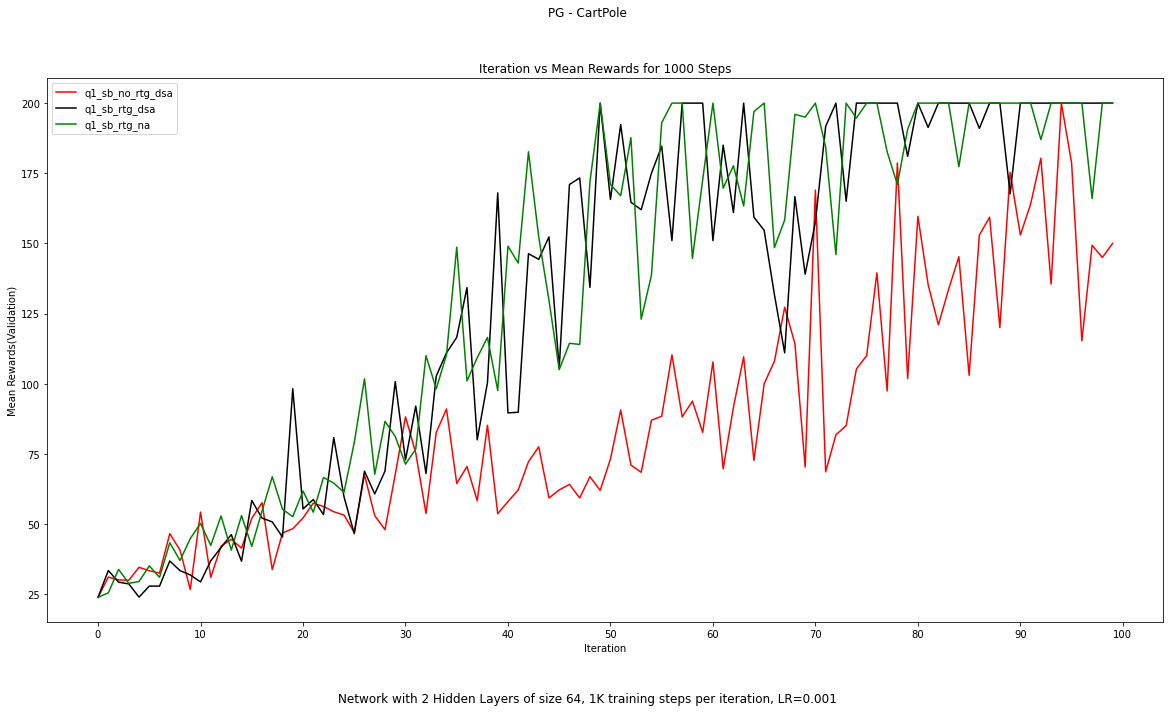
\includegraphics[scale=0.35]{q1_sb_plot}

    Reward-to-go estimator performs better.
    Advantage standardization difference is not statistically significant.


    \hspace*{-0.5in}
    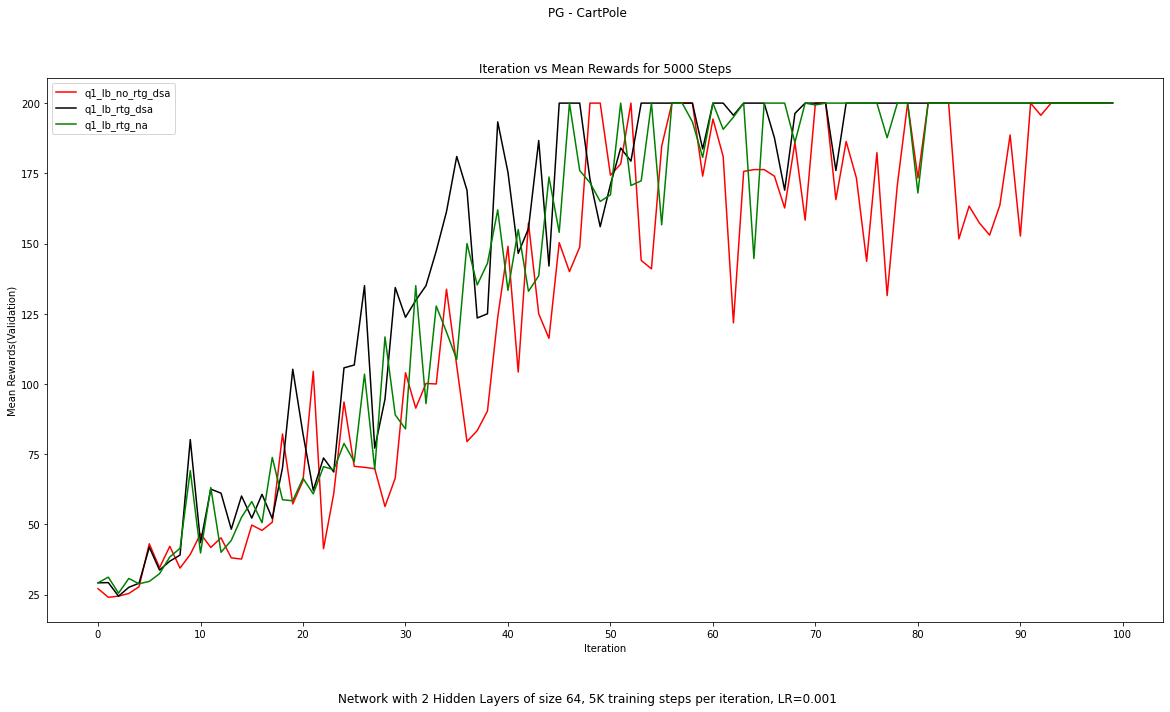
\includegraphics[scale=0.35]{q1_lb_plot}

    Reward-to-go estimator performs better.
    Advantage standardization difference is not statistically significant.
    Increasing batch size helps the algorithm converge with fewer iterations.


\end{document}